%% Forward-model validation of an AFM tip-convolution simulator against real Bruker scans.
%% Elsevier elsarticle template. Build: latexmk -pdf main.tex   (or: tectonic main.tex)
\documentclass[preprint,12pt]{elsarticle}

\usepackage{amsmath,amssymb}
\usepackage{graphicx}
\usepackage{booktabs}
\usepackage{siunitx}
\usepackage{xcolor}
\usepackage[hidelinks]{hyperref}
\usepackage{lineno}
\usepackage{tikz}
\usetikzlibrary{positioning,arrows.meta,fit}

\sisetup{range-phrase=--,range-units=single,separate-uncertainty=true}
\newcommand{\tagm}{\textsc{[meas]}}
\newcommand{\tags}{\textsc{[sim]}}
\newcommand{\tagi}{\textsc{[inf]}}
\newcommand{\todo}[1]{\textcolor{red}{[TODO: #1]}}

\journal{Ultramicroscopy}

\begin{document}

\begin{frontmatter}

\title{What a geometric tip-convolution simulator can and cannot predict:\\
held-out validation against real AFM scans of calibration standards}

%% TODO: replace with the real author list, order and affiliations.
\author[isu]{First Author\corref{cor1}} % TODO: real name
\ead{alloydas@iastate.edu}
\author[isu]{Avish Cooray} % TODO: confirm name, role, affiliation
\author[isu]{Further Authors} % TODO: supervisors / co-authors
\cortext[cor1]{Corresponding author}
\affiliation[isu]{organization={Department (TODO), Iowa State University},
            city={Ames},
            state={IA},
            country={USA}}

\begin{abstract}
Atomic force microscopy (AFM) images are the sample topography dilated by the finite probe, and
grey-scale morphological dilation is the standard geometric model of this effect. Simulators built
on it are increasingly used to generate training data and benchmarks for tip deconvolution, yet
they are rarely tested against real measurements under a protocol that separates what the data can
validate from what they cannot. We present an open, browser-based and Python AFM forward simulator
and validate it against 70 Bruker image files from ten folders recorded on two instruments
(Dimension Icon and BioScope Resolve) on gratings, a step standard with a sphere probe, polymer
films and fused silica. Each real frame is simulated on its own pixel grid with every candidate
probe model. Sample geometry is calibrated on designated frames and transferred unchanged to
held-out frames, and every reported claim was re-checked by three independent verification passes.
The Python engine reproduces the browser page bit for bit over 73,410 configurations. On five
grating folders, a measured rounded-square-pit model reproduces the held-out frames to
2.8--6.3~nm RMS (1.6--5.1\,\% of the 171--185~nm step), against 25--50~nm for the nominal sample
presets, with 82--99\,\% of the misfit on the pit walls. The probe radius stated in the file header
is not a usable simulator input: a 10~\si{\micro\metre} sphere is rejected by 52--80~nm step-edge
widths, and an effective radius of at most about 150~nm follows only if the instrument's
one-pixel fast-axis response is modelled. Conversely, none of these samples identifies the tip at
the nominal radius scale ($R \lesssim 12$~nm), the yaw sign, or the absolute $XY$/$Z$ calibration.
We report these limits explicitly as the boundary conditions for inverse-problem benchmarks built
on such simulators.
\end{abstract}

\begin{keyword}
atomic force microscopy \sep tip convolution \sep morphological dilation \sep forward model
\sep validation \sep calibration gratings \sep blind tip reconstruction
\end{keyword}

\end{frontmatter}

\linenumbers

%% =====================================================================
\section{Introduction}
\label{sec:intro}

The atomic force microscope~\cite{binnig1986} records topography by scanning a sharp probe over a
surface. Because the probe has a finite size and shape, the image is not the surface: narrow
trenches are inaccessible, sharp features are broadened and rounded, and damaged or multi-apex
probes produce duplicated features. In the height-field approximation this tip--sample
interaction is grey-scale morphological dilation of the surface by the reflected tip, and
erosion with a known tip gives the tightest surface consistent with the image~\cite{keller1991,
villarrubia1997}. Villarrubia's algorithms for image simulation, surface reconstruction, blind tip
reconstruction (BTR) and certainty maps~\cite{villarrubia1997} are implemented in standard analysis
software such as Gwyddion~\cite{necas2012,gwyddionguide}.

Forward simulators built on this model have gained a second role: generating paired
true/measured data for learned restoration and tip estimation. Convolutional networks trained on
synthetic distorted/ground-truth pairs correct AFM artefacts~\cite{kocur2023} and recover nanoscale
profiles~\cite{bonagiri2024}; differentiable dilation and erosion make BTR robust to
noise~\cite{matsunaga2023}; synthetic generators with tip convolution, noise, debris and feedback
artefacts train models for autonomous AFM~\cite{millansolsona2026}; and multi-view neural
reconstruction models commercial pyramidal tips parametrically~\cite{chen2024}. Independent tip
characterisation by electron microscopy, critical-dimension AFM or reference
trenches~\cite{dai2020,trench2025} provides the probe ground truth these methods need.

All of these uses assume that the simulator reproduces real images when it is given the right
sample and probe. That assumption is seldom tested directly against real scans, and when it is,
the test rarely states what the data could not have revealed. A pixel-level agreement on a
grating, for example, may say nothing about the tip if the grating walls are shallower than every
probe facet. This distinction matters for inverse-problem benchmarks: a simulator validated only
where the tip is invisible cannot certify tip-dependent conclusions.

This paper reports such a validation. Its contributions are:
\begin{enumerate}
  \item an open forward simulator (interactive 2D and 3D browser applications and a vectorised
        Python engine) whose engine is shown to reproduce the browser page bit for bit
        (Section~\ref{sec:model});
  \item a validation protocol for real Bruker data with a case catalogue, explicit
        calibrate/predict roles, candidate-probe sweeps, a no-tip control and an evidence tag on
        every number (Section~\ref{sec:methods});
  \item held-out results on ten folders of real data, with each headline claim re-checked by
        three independent verification passes (Section~\ref{sec:results}); and
  \item an explicit list of what these measurements validate and what they cannot, which sets
        the boundary conditions for the inverse problem (Section~\ref{sec:discussion}).
\end{enumerate}

%% =====================================================================
\section{Forward model and implementation}
\label{sec:model}

\subsection{Imaging model}

A surface is a height field $S(\mathbf{x})$ over lateral positions $\mathbf{x}=(x,y)$, and a probe
is represented by its lower height envelope $T(\mathbf{d})\ge 0$, the height of the tip above its
apex at lateral offset $\mathbf{d}$, with $T(\mathbf{0})=0$. Contact-mode imaging is computed as
dilation,
\begin{equation}
  I(\mathbf{x}) = \max_{\mathbf{d}} \bigl[\, S(\mathbf{x}+\mathbf{d}) - T(\mathbf{d}) \,\bigr],
  \label{eq:dilation}
\end{equation}
and the classical reconstruction with a known tip is the erosion
\begin{equation}
  E(\mathbf{x}) = \min_{\mathbf{d}} \bigl[\, I(\mathbf{x}-\mathbf{d}) + T(\mathbf{d}) \,\bigr],
  \label{eq:erosion}
\end{equation}
which is an upper bound on $S$ and equals it only where the tip touched the surface at a single
point~\cite{villarrubia1997}. Forward imaging always uses Eq.~\eqref{eq:dilation}, also for the
concave probe model; erosion is available only as an explicit inverse option.

The model is geometric. It does not represent cantilever dynamics, feedback control, adhesion,
friction, sample or tip deformation, or overhanging surfaces. These boundaries are deliberate and
are part of what Section~\ref{sec:results} tests. Figure~\ref{fig:concept} illustrates the model
on a synthetic profile.

\begin{figure}[t]
\centering
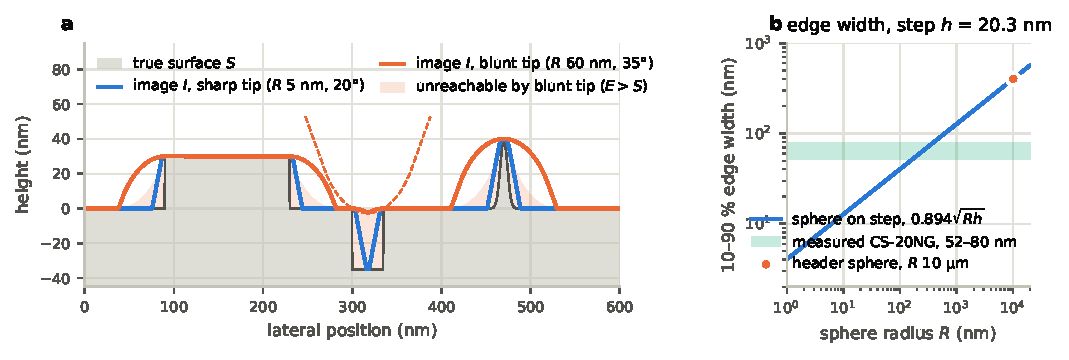
\includegraphics[width=\textwidth]{figures/fig_concept.pdf}
\caption{The imaging model. (a) A synthetic profile (grey) imaged by Eq.~\eqref{eq:dilation} with a
sharp sphere--cone tip ($R=5$~nm, $20^\circ$ half-angle, blue) and a blunt one ($R=60$~nm,
$35^\circ$, orange; dashed: the tip at the trench centre). The blunt tip cannot enter the 35~nm
trench and broadens the asperity. Shaded: where the erosion $E$ of the blunt-tip image
(Eq.~\eqref{eq:erosion}) lies above the true surface, i.e.\ surface the tip never reached.
(b) 10--90\,\% edge width of a sphere on a 20.3~nm step, Eq.~\eqref{eq:edge}, against the radius.
The edge widths measured on CS-20NG (52--80~nm, Section~\ref{sec:cs20ng}) are 5--8 times narrower
than the 403~nm the header's 10~\si{\micro\metre} sphere implies. The closed form ignores the
instrument's pixel response, so it does not by itself give the radius.}
\label{fig:concept}
\end{figure}

\subsection{Probe and surface libraries}

The analytical probe library contains conical, spherical, hyperboloidal, flat-punch, concave
(inverse sphere), asymmetric, double-tip and combined sphere--cone tips. The 3D application adds a
faceted pyramid with unequal front, back and side angles and a rounded apex, with default
dimensions taken from a commercial probe specification. Probe meshes for the probes used in this
study (RTESPA, ScanAsyst-Air, SNL-10 and SAA-SPH) are generated as Wavefront OBJ files. An
independent tool checks them by casting vertical rays against the triangles and comparing the
resulting lower envelope with the analytical tip equation. The surface library ranges from
periodic waves, particles, pits and trenches to rough, chirped and lattice surfaces, plus models
of the calibration samples used here (Section~\ref{sec:samples}). Imported OBJ meshes are
rasterised to their upper envelope (surfaces) or lower envelope (probes).

\subsection{Implementations}

\paragraph{Browser applications} A 2D line-scan simulator and a 3D raster simulator are written as
static HTML/JavaScript (Three.js rendering). The 3D page computes an $80\times80$ height map and
exports true and measured maps (CSV and 16-bit PNG), parameters, metadata and OBJ meshes. The
animated probe is only a visualisation layer: the measured map is always computed from the full
discrete dilation.

\paragraph{Python engine} \texttt{afm\_forward\_sim} has two layers. The \emph{parity layer}
reproduces the page's computation on its $80\times80$ grid, including its kernel truncation and
height clamp. The \emph{physical layer}, used for every real-scan simulation in this paper, applies
the same tip and surface geometry on arbitrary grids. It dilates on a fine grid of spacing
$\Delta/u$ (pixel size $\Delta$, upsampling $u\ge 8$ in full runs) and point-samples at pixel
centres. Vertical grating walls are dilated exactly from their outlines; sloped walls go through
the fine lattice, whose error falls roughly as $1/u$. For apex radii beyond the page's lookup
table ($R>12$~nm), pyramids use the exact morphological opening by the apex ball.

\paragraph{Parity} A test harness drives the 3D page in headless Chrome: it clicks the same
buttons and moves the same sliders as a user, pins the random seed and reads back every
intermediate array. Over 73,410 configurations of tip, surface, scan size, slider extremes,
toggles and noise, the parity layer matched the page with zero mismatches and a maximum absolute
difference of 0~nm \tags. Parity shows that the page and the engine model the same geometry. It
does not show that the page's $80\times80$ grid can reproduce real scans; that is the physical
layer's role.

%% =====================================================================
\section{Validation data and methods}
\label{sec:methods}

\subsection{Data}
\label{sec:samples}

Table~\ref{tab:data} lists the ten data folders. They were recorded in PeakForce Tapping mode on a
Bruker Dimension Icon and a Bruker BioScope Resolve, on two square-pit gratings (VGRP-15M, VGRP-GS),
a step standard (CS-20NG), a three-dimensional grating (TGXYZ02), two polymer films (PSFILM-12M,
PS-LDPE-12M) and fused silica (FSILICA-12M). Of the 70 image files, 51 were simulated and compared.
The case catalogue excluded 19, each with a stated reason (for example feedback oscillation, drift
shear or a wrong header scan size). A machine-readable case catalogue records, for every folder,
the instrument, decoding conventions, nominal and measured sample models, candidate probe models,
the role of every scan and the known artefacts.

\begin{table}[t]
\centering
\caption{Data folders. Probe: folder label and file-header values, which were not independently
checked. Frames: compared / catalogue files. Class: analysis driver.}
\label{tab:data}
\small
\resizebox{\textwidth}{!}{%
\begin{tabular}{@{}llllcl@{}}
\toprule
Sample & Instr. & Probe label & Header probe & Frames & Class \\
\midrule
FSILICA-12M & Icon    & ScanAsyst Air Probe2 & ScanAsyst-Air, $R$ 5 nm      & 5/11 & flat reference \\
PSFILM-12M  & Icon    & ScanAsyst Air Probe2 & ScanAsyst-Air, $R$ 5 nm      & 17/17 & polymer \\
PS-LDPE-12M & Resolve & ScanAsystAir         & $R$ 5 nm                     & 8/8  & polymer \\
VGRP-15M    & Icon    & RTESPA 300 Probe2    & RTESPA-300-125, $R$ 125 nm   & 4/5  & grating \\
VGRP-15M    & Icon    & ScanAsyst Air Probe4 & ScanAsyst-Air, $R$ 5 nm      & 6/6  & grating \\
VGRP-GS     & Resolve & RTESPA-150           & $R$ 8 nm                     & 2/10 & grating \\
VGRP-GS     & Resolve & ScanAsystAir         & $R$ 5 nm                     & 3/4  & grating \\
VGRP-15M    & Resolve & SNL10 B              & $R$ 8 nm, $k$ 42 N/m         & 3/4  & grating \\
CS-20NG     & Icon    & SAA\_SPH\_10UM Probe4 & SAA-SPH-10UM, $R$ 10 \si{\micro\metre} & 3/3 & sphere edges \\
TGXYZ02     & Icon    & SAA\_SPH\_10UM Probe4 & SAA-SPH-10UM, $R$ 10 \si{\micro\metre} & 0/2 & negative control \\
\midrule
\multicolumn{4}{@{}l}{Total} & 51/70 & \\
\bottomrule
\end{tabular}}
\end{table}

\subsection{Decoding, masks and conventions}

Height channels are decoded following Gwyddion's NanoScope importer: height = raw $\times$ HV
$/\,2^{8B}\times S$, with raw the signed little-endian integer at the stored width, HV the hard
value of the $Z$ scale, $B$ the declared bytes per pixel and $S$ the sensitivity. The reader is
bit-identical to reference decoders on all 136 files tested \tagm. The metrology channel is the
Height Sensor, because the Height (piezo drive) channel reads 0.4--2.5\,\% high and carries creep
and hysteresis \tagm. Arrays are kept in stored order and pixel $(i,j)$ is centred at
$(x,y)=(j\Delta_x, i\Delta_y)$ with $\Delta = L/N$ for scan size $L$ and $N$ pixels.

No metric uses an invalid pixel. Masks combine zero-filled dropout runs, catalogue-listed
corrupted segments, and rows rejected by the registration; railed channels are flagged and never
read as topography.

\subsection{Levelling, registration and sample models}

Images are levelled with robust plane and per-line fits on a reference-level mask; for gratings a
two-level segmentation (Otsu thresholding~\cite{otsu1979} with morphology) defines that mask. A
square lattice is registered in three steps: an FFT estimate, least squares on feature centroids,
and a model-image fit of rounded rectangles with a linear wall and Gaussian blur. The result is the
full lattice affine (per-axis scale and shear), which places the sample model in image
coordinates. In synthetic round trips this registration leaves a model floor of small wall and
corner deltas and a 0.3--0.9~nm depth bias \tags.

Each grating has three sample models:
\begin{description}
  \item[M0] the simulator's built-in preset: 5~\si{\micro\metre} sharp, vertical-walled pits;
  \item[M1] an earlier hand-built model of 6~\si{\micro\metre} wells;
  \item[M2] a measured rounded-square-pit model with six parameters (depth, two half-widths,
        corner radius, wall run and wall blur), calibrated through the simulator on the
        folder's \emph{calibrate} frames only.
\end{description}
On each \emph{predict} frame, M2 is transferred unchanged and only that frame's registration and
levelling are refitted; this is the held-out comparison M2\textsubscript{holdout}. The
calibration is probe-consistent: it is repeated for every probe hypothesis, so the geometry is the
one that, dilated by that probe, best matches the calibrate frames. A cross-probe pair (same
sample, instrument and mounting, two probes) fits the geometry on one probe's frames and predicts
the other's. Figure~\ref{fig:workflow} summarises the pipeline.

\begin{figure}[t]
\centering
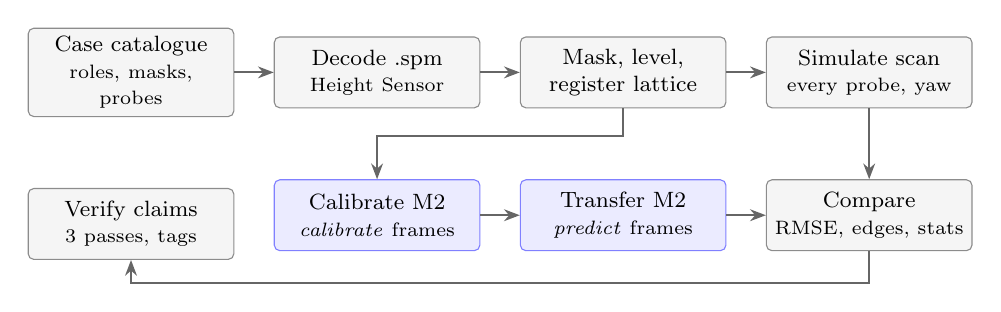
\begin{tikzpicture}[
  node distance=4mm and 5mm, font=\footnotesize,
  box/.style={draw=black!45, rounded corners=2pt, fill=black!4, align=center,
              minimum height=9mm, text width=24mm, inner sep=3pt},
  key/.style={box, fill=blue!8, draw=blue!50},
  arr/.style={-{Stealth[length=2mm]}, black!60, thick}]
  \node[box] (cat) {Case catalogue\\\scriptsize roles, masks, probes};
  \node[box, right=of cat] (dec) {Decode .spm\\\scriptsize Height Sensor};
  \node[box, right=of dec] (lev) {Mask, level,\\register lattice};
  \node[box, right=of lev] (sim) {Simulate scan\\\scriptsize every probe, yaw};
  \node[key, below=9mm of dec] (cal) {Calibrate M2\\\scriptsize \emph{calibrate} frames};
  \node[key, right=of cal] (tr) {Transfer M2\\\scriptsize \emph{predict} frames};
  \node[box, right=of tr] (cmp) {Compare\\\scriptsize RMSE, edges, stats};
  \node[box, below=9mm of cat] (ver) {Verify claims\\\scriptsize 3 passes, tags};
  \draw[arr] (cat) -- (dec);
  \draw[arr] (dec) -- (lev);
  \draw[arr] (lev) -- (sim);
  \draw[arr] (lev.south) |- ++(0,-3.5mm) -| (cal.north);
  \draw[arr] (cal) -- (tr);
  \draw[arr] (tr) -- (cmp);
  \draw[arr] (sim.south) -- (cmp.north);
  \draw[arr] (cmp.south) |- ++(0,-4mm) -| (ver.south);
\end{tikzpicture}
\caption{Validation pipeline. The case catalogue fixes every scan's role before any fit. The
measured sample model M2 is calibrated through the simulator on \emph{calibrate} frames only and
transferred unchanged to \emph{predict} frames, where only the registration and levelling are
refitted. Each frame is simulated with every candidate probe, both yaw signs and a no-tip control.
Every reported claim then carries an evidence tag and passes three verification lenses.}
\label{fig:workflow}
\end{figure}

\subsection{Probe hypotheses, orientation and sampling}

Every probe hypothesis in the catalogue is simulated: header values, folder-label values, radius
sweeps (2--250~nm) and a no-tip control, which isolates the tip's contribution. The engine's tip
frame has the cantilever axis across the fast scan at yaw $0^\circ$; at Bruker scan angle 0 the
fast axis runs along the cantilever, so the physical geometry is yaw $\pm 90^\circ$
\tagi. The sign is not established, so both signs and the yaw-$0^\circ$ control are simulated and
reported; a yaw selected by a residual is a fit, not a measurement.

The simulation point-samples each pixel, while the instrument averages 2.0--15.1 PeakForce cycles
per pixel along the fast axis \tagm. Where a driver models this fast-axis pixel response, it says
so, and Section~\ref{sec:cs20ng} shows where the choice matters.

\subsection{Metrics}

For registered samples the residual is $r = I_\text{sim} - I_\text{meas}$ on valid pixels, with no
fitted offset, and
\begin{equation}
  \text{RMSE} = \Bigl(\tfrac{1}{N}\textstyle\sum r^2\Bigr)^{1/2}.
\end{equation}
It is split into a wall band (pixels within the wall extent plus two pixels of the registered
outline) and the remaining flat pixels. Tip discrimination within a folder is the largest
image difference between any two probe hypotheses, each after its probe-consistent calibration,
divided by the scan's residual floor. A value below 1 means that the hypotheses cannot be told
apart. For the step standard we use 10--90\,\% edge widths and joint fits of geometry,
fast-axis response and sphere radius. A sphere of radius $R$ imaging a vertical step of height
$h$ gives a 10--90\,\% edge width
\begin{equation}
  w_{10\text{--}90} = \bigl(\sqrt{1.8}-\sqrt{0.2}\bigr)\sqrt{Rh} \approx 0.894\sqrt{Rh},
  \label{eq:edge}
\end{equation}
and walls steeper than about $4^\circ$ cannot make it narrower. The random-surface presets of
the polymer and fused-silica samples are not registered to the real topography, so those samples
are compared statistically (background $S_q$, autocorrelation length, power spectral density and
feature statistics). They are also compared in a cross-scale test: a measured finer zoom is
resampled through the engine onto its parent frame.

\subsection{Evidence tags and verification}

Every reported number carries a basis tag: \tagm{} (derived from the measured images alone),
\tags{} (from the simulator, alone or compared with a measurement) or \tagi{} (a conclusion drawn
from both). Each run records checksums of its inputs (engine, modules, catalogue, driver) so that
results from older code are flagged, never presented as current. The four main claims of each
folder (40 in total) were then checked by three independent verification passes: \emph{reproduce}
(re-derive the numbers from the outputs and from the raw files with independent code),
\emph{method} (circularity, conventions, uncertainty) and \emph{scope} (wording strength,
alternative explanations). None of the 40 claims was refuted. All 40 required qualification of
scope, uncertainty or wording, and the statements below use the qualified versions. A separate
report recomputed 22,596 reported values from the saved maps; all matched within 0.01~nm.

%% =====================================================================
\section{Results}
\label{sec:results}

\subsection{Gratings: the measured sample model transfers to held-out frames}

Table~\ref{tab:gratings} and Fig.~\ref{fig:vgrp} summarise the five grating folders. With the
folder-label probe, M2\textsubscript{holdout} reproduces the held-out frames to 2.8--6.3~nm RMS per
folder (single frames 2.8--8.8~nm, 1.6--5.1\,\% of the 171--185~nm step) \tags. The nominal preset
M0 leaves 31--50~nm and M1 25--49~nm, 5--18 times more. These baselines show that the nominal pit
size, vertical walls and sharp corners are wrong; they do not measure predictive skill.

\begin{table}[t]
\centering
\caption{Grating results with the folder-label probe at yaw $+90^\circ$ \tags. Held-out: number of
predict frames (independent sites). RMSE: mean (range) over held-out frames. Discr.: tip
discrimination ratio ($<1$: probe hypotheses indistinguishable). Depth: measured step, mean
$\pm$ SE over frames \tagm.}
\label{tab:gratings}
\small
\resizebox{\textwidth}{!}{%
\begin{tabular}{@{}lcccccc@{}}
\toprule
Folder & Held-out & M2\textsubscript{holdout} (nm) & M0 (nm) & M1 (nm) & Discr. & Depth (nm) \\
\midrule
VGRP-15M Icon, ScanAsyst-Air & 3 (3) & 3.45 (3.15--4.03) & 49.6 & 25.9 & 0.089 & $184.54\pm0.06$ \\
VGRP-15M Icon, RTESPA-300    & 3 (2) & 4.91 (4.67--5.08) & 49.5 & 25.8 & 0.61  & $184.07\pm0.06$ \\
VGRP-GS Resolve, RTESPA-150  & 1 (1) & 2.79              & 31.0 & 49.2 & 0.13  & $171.04\pm0.09$ \\
VGRP-GS Resolve, ScanAsyst-Air & 1$^a$ & 3.93$^b$        & 32.6 & 45.5 & 0.12  & $171.94\pm0.06$ \\
VGRP-15M Resolve, SNL10 B    & 2$^c$ & 6.34 (3.84--8.84) & 47.5 & 31.0 & 0.16  & $174.68\pm0.02$ \\
\bottomrule
\end{tabular}}

\smallskip
\raggedright\footnotesize
$^a$ Weak hold-out: same site as a calibrate frame, probably the same pits.
$^b$ 3.59~nm with PeakForce pixel averaging.
$^c$ One field imaged twice.
\end{table}

\begin{figure}[t]
\centering
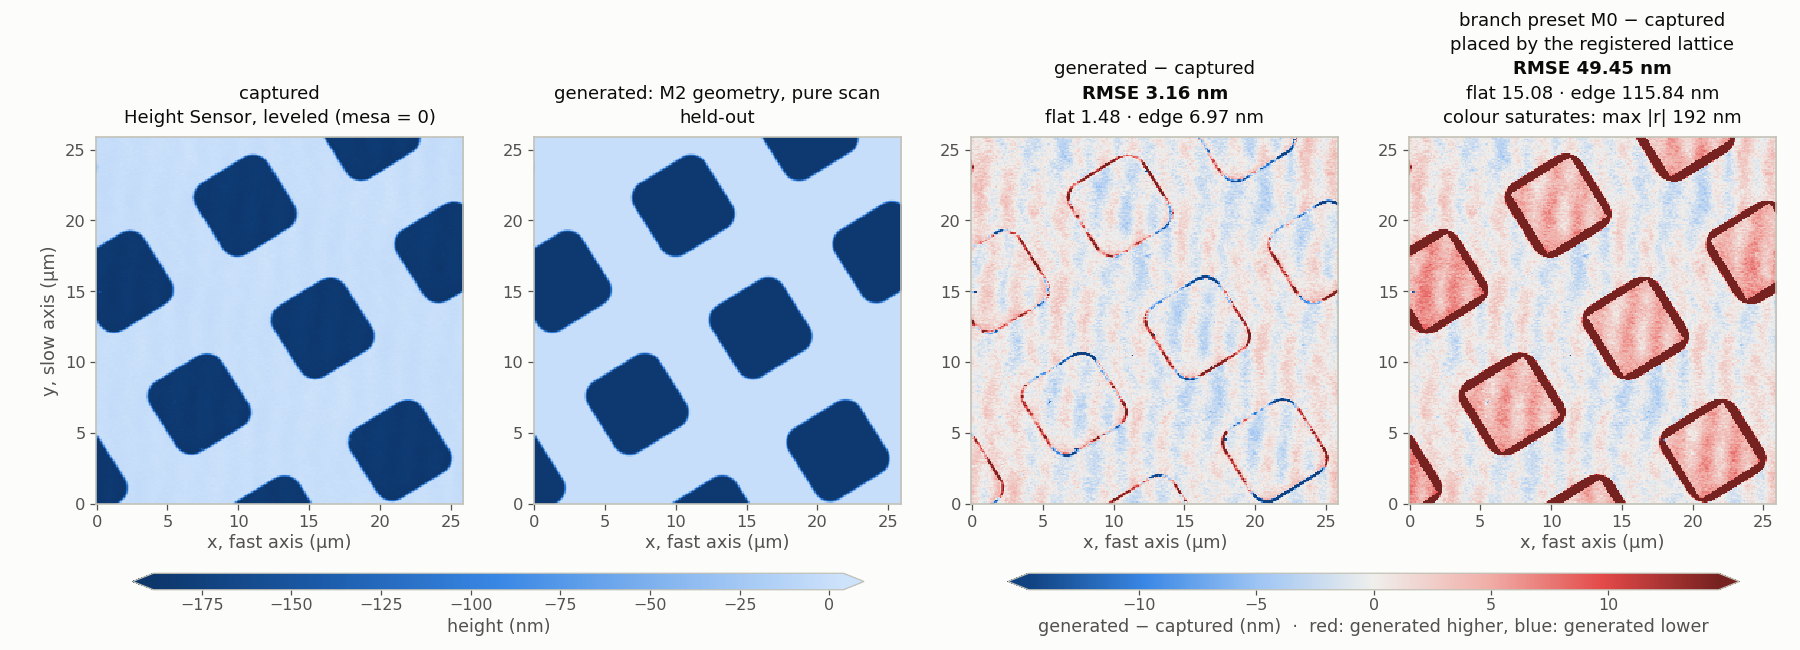
\includegraphics[width=\textwidth]{figures/vgrp_probe4_heldout.png}
\caption{Held-out prediction on VGRP-15M (Dimension Icon, ScanAsyst-Air probe, frame 00004,
$256\times256$ pixels at 101.3~nm/pixel). From left: measured Height Sensor image (levelled, mesa
$=0$); the pure simulated scan of the M2 geometry calibrated on other frames at another site;
simulated minus measured (RMSE 3.16~nm; flat 1.48~nm, wall 6.97~nm); the same for the nominal
preset M0 placed by the registered lattice (RMSE 49.45~nm). The difference colour scale is
clipped at 14.7~nm.}
\label{fig:vgrp}
\end{figure}

The Icon VGRP-15M folder with the ScanAsyst-Air probe is the strongest case. Its calibrate frames
come from one stage site, and its three held-out frames from three non-overlapping sites
0.65--1.07~mm away. The probe-consistent calibration gives half-depth widths of
$5770\times5793$~nm, 1187~nm corner radii, a 184.60~nm depth and a 152~nm 10--90\,\% wall.
Transferred unchanged, it reproduces the held-out frames at 4.03, 3.16 and 3.15~nm
(mean $3.45\pm0.29$~nm, SE over sites). Calibrating the same model on each held-out frame itself
improves this by only 0.05--0.36~nm, and leave-one-site-out calibration gives site means of
3.47--3.67~nm \tags.

The residual sits on the walls. The wall band holds 12--18\,\% of the pixels but 82--87\,\% of the
squared residual (band RMSE 6.8--10.9~nm). The flat-region RMSE (mean 1.455~nm) equals the frames'
own flat-level scatter (1.454~nm). That equality holds for any flat model with the correct depth,
so it confirms only the transferred depth, not the lateral geometry \tagi. Figure~\ref{fig:gratings}
shows the same pattern on every held-out grating frame.

\begin{figure}[t]
\centering
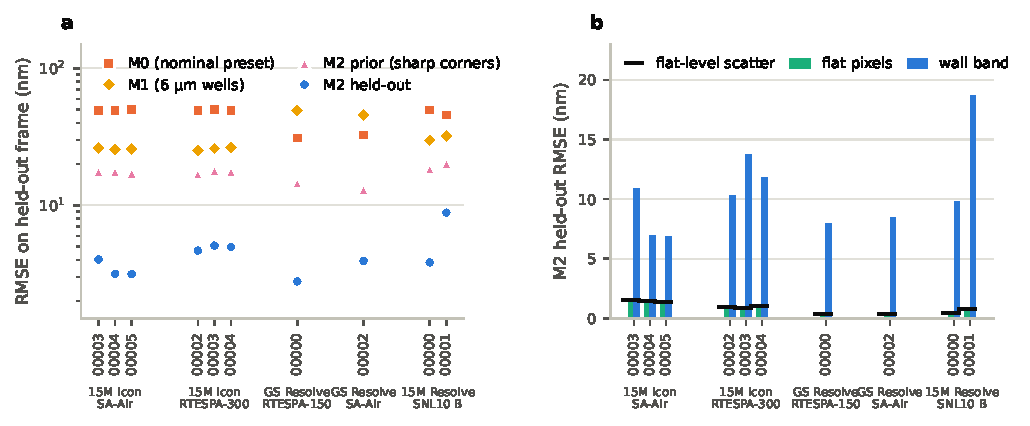
\includegraphics[width=\textwidth]{figures/fig_gratings.pdf}
\caption{All ten held-out grating frames (label probe, yaw $+90^\circ$), grouped by folder in the
order of Table~\ref{tab:gratings}. (a) RMSE of the three sample models (log scale): the
transferred measured model M2 against the nominal preset M0, the 6~\si{\micro\metre} wells M1
and the catalogue prior with sharp corners. (b) M2 held-out RMSE on the flat pixels and in the
wall band, with each frame's own flat-level scatter. The flat error is at or below the scatter on
every frame; the misfit is on the walls.}
\label{fig:gratings}
\end{figure}

The remaining wall misfit comes from effects the model omits, not from the tip:
\begin{itemize}
  \item open-loop fast-axis scanner non-linearity, about 0.4\,\% per 10~\si{\micro\metre}
        (RTESPA-150);
  \item drift shear (VGRP-GS);
  \item PeakForce feedback on fast-axis walls (SNL10 B; 15.5~nm on its fast calibrate frame);
  \item site- and session-dependent pit widths (the RTESPA-300 held-out pits image 2--55~nm
        narrower; cause not identified).
\end{itemize}

\paragraph{The tip is not identifiable on the gratings} Every probe hypothesis, the no-tip control
included, gives the same held-out RMSE to within 0.05~nm on three of the five folders (for
example 3.447~nm without a tip and 3.459~nm with $R=12$~nm). The discrimination ratio is below 1
in every folder (0.089--0.61). The reason is geometric: the 43--49$^\circ$ pit walls are
shallower than every probe facet, and the
probe-consistent calibration absorbs the apex into the pit width. With the geometry held fixed,
dilation by $R=125$--250~nm is visible (up to 19.4~nm RMS) but disappears after recalibration
(1.6~nm). The raw fixed-geometry difference is therefore not a discrimination test \tags.
Figure~\ref{fig:tip} shows this on the two Icon VGRP-15M folders. With the nominal geometry held
fixed, a larger apex raises the held-out RMSE by up to 10.8~nm ($R=250$~nm). After the
probe-consistent recalibration, the same probes change it by at most 0.52~nm on the RTESPA-300
folder and 0.011~nm on the ScanAsyst-Air folder.

\begin{figure}[t]
\centering
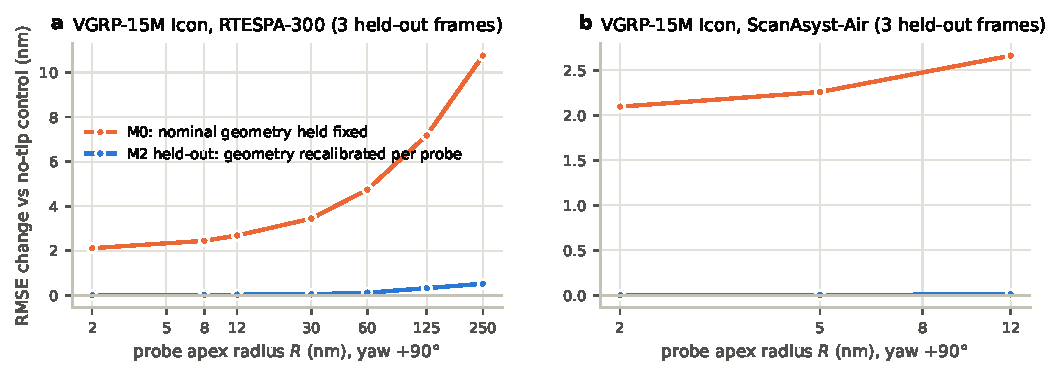
\includegraphics[width=\textwidth]{figures/fig_tip.pdf}
\caption{Why the gratings do not identify the tip. Change of the held-out RMSE relative to the
no-tip control, mean over the three held-out frames, against the simulated apex radius:
(a) VGRP-15M Icon, RTESPA-300 folder (no-tip control: M0 47.09~nm, M2 4.89~nm); (b) VGRP-15M
Icon, ScanAsyst-Air folder (M0 47.52~nm, M2 3.448~nm). Orange: nominal geometry held fixed, so the
dilation is visible. Blue: the measured geometry recalibrated for each probe absorbs the apex into
the pit width. The ranking along the blue line is not tip evidence.}
\label{fig:tip}
\end{figure}

\paragraph{Cross-probe pair} Only the Icon VGRP-15M pair tests the geometry that each probe
hypothesis implies. Relative to a ScanAsyst-Air apex near its nominal radius, the header's
125~nm apex for the RTESPA-300 probe is inconsistent with the pit widths in a post-hoc
site-level two-sample test (9.4 SE, $p=2.3\times10^{-4}$), while radii up to about 30~nm are
consistent \tagi. The pre-registered decision rule returns only ``mixed'' for this hypothesis,
because with three or four target sites its pooled-$t$ critical values (19.2 and 9.22) are out of
reach. The test therefore lacks power; it is not conflicting evidence. Neither the pair nor the
folder singles out $R=8$~nm.

\paragraph{Instrument readings} Within a session the step depth repeats to an SE of
0.02--0.09~nm over frames \tagm. Between probes on the same die the depth differs by 0.47~nm (Icon) and 0.95~nm (Resolve).
The Resolve reads the VGRP-15M depth at 0.947--0.949 of the Icon's, although it is unknown
whether the two instruments imaged the same die \tagm. These are session values, not traceable
calibrations: the 180~nm nominal depth has no stated tolerance, and every pitch was assumed exact.

\subsection{Step standard: header tip metadata is not a valid simulator input}
\label{sec:cs20ng}

The CS-20NG frames were recorded with a probe whose header names a 10~\si{\micro\metre} sphere
(SAA-SPH-10UM). For the measured 19.9--20.4~nm steps, Eq.~\eqref{eq:edge} and the engine both
predict 10--90\,\% edges of about 400~nm \tags. The measured edges are 52--80~nm, or 42--117~nm
across the estimators and edge families tried, which is 3.4--10 times narrower and close to the
one-pixel sampling floor \tagm (Fig.~\ref{fig:cs20ng}). Pixel averaging, feedback lag, drift,
calibration, yaw or holder tilt can only widen the predicted edge, so none of them closes the
gap. Joint fits that refit geometry, wall and fast-axis response at each radius reject
$R=10$~\si{\micro\metre} in every variant: the pooled paired $t$ is 21.8--22.0 over 309 edge
segments, and 3.55 against a critical 2.92 with the frame as the statistical unit \tagi.

\begin{figure}[t]
\centering
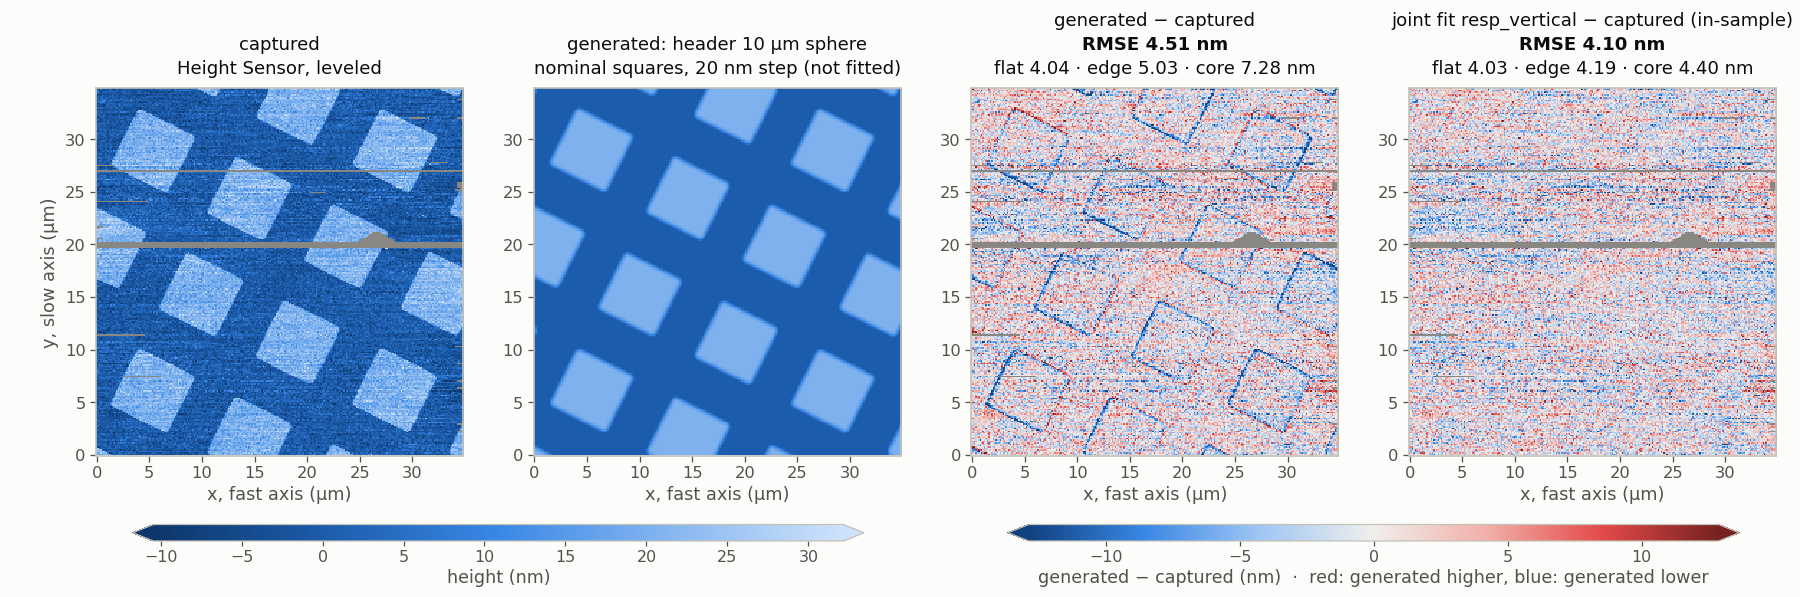
\includegraphics[width=\textwidth]{figures/cs20ng_sphere.png}
\caption{CS-20NG step standard (Icon, frame 00000, 136.3~nm/pixel). From left: measured image;
the forward prediction with the header's 10~\si{\micro\metre} sphere on the nominal squares
(placement registered, nothing else fitted); its residual (RMSE 4.51~nm); the residual of the
in-sample joint fit of geometry, fast-axis response and a sphere radius pooled over three frames
(RMSE 4.10~nm). Grey: masked pixels of the captured frame (dropout rows, particles), not
compared; the generated map is the pure, unmasked scan. The 10~\si{\micro\metre} sphere is rejected by the edge widths, not by these
image RMSEs: its 0.9~\si{\micro\metre} broadening partly offsets the nominal-width error.}
\label{fig:cs20ng}
\end{figure}

The effective radius is bounded only conditionally. With the instrument's fast-axis response
modelled (a box about one pixel wide, consistent with averaging over the 3.91~ms dwell of 7.8
PeakForce cycles), the three frames give a conservative upper bound of about 150~nm on the
sphere-equivalent apex radius over the bottom 20~nm of the probe. The bracket is 130--153~nm
across accepted variants; the best fits are 76--95~nm, and there is no lower bound \tagi. The
simulator's own pixel-centre sampling is rejected (paired $t=8.9$): it cannot reproduce the
measured fast/slow edge anisotropy (for example 117/65~nm), and with it the bound would be
476~nm. The tip-radius conclusion therefore depends on modelling the pixel response, while the
rejection of the header radius does not. The data cannot distinguish a sharp probe from a
10~\si{\micro\metre} sphere carrying an asperity or debris particle protruding about 20~nm, which
would give 24--59~nm edges \tags.

Nominal-geometry image RMSEs rank the probes wrongly: they favour the 10~\si{\micro\metre}
sphere. Only geometry-refitted fits rank probes correctly. Figure~\ref{fig:cs20ngedges} shows the
edge evidence directly.

\begin{figure}[t]
\centering
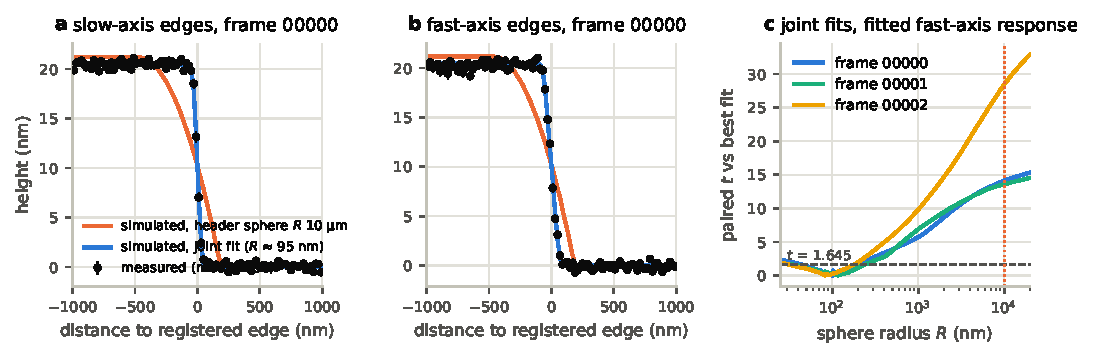
\includegraphics[width=\textwidth]{figures/fig_cs20ng.pdf}
\caption{CS-20NG edge evidence. (a, b) Mean edge profiles of frame 00000 against the distance to
the registered outline, for edges crossing the slow and the fast scan axis: measured (mean $\pm$
SE per 20~nm bin), the joint fit with the header's 10~\si{\micro\metre} sphere, and the best joint
fit (fitted fast-axis response; $R\approx95$~nm pooled). (c) Paired segment $t$ of each radius
against the best fit, per frame, for the same model. The header radius (dotted) is rejected on
every frame ($t$ 13.6--28.5). Single frames bound the radius at 193, 248 and 180~nm; the pooled
bound is 153~nm, and it holds only with the fast-axis response modelled.}
\label{fig:cs20ngedges}
\end{figure}

\subsection{Polymers and fused silica: statistics and cross-scale consistency}

The random-surface presets for these samples are not registered to the real topography, so only
statistics can be compared, and each preset fails in a specific way \tagi:
\begin{itemize}
  \item the fused-silica preset ($S_q$ roughness 0.3~nm) is 26--54\,\% too smooth (ratio 0.46--0.74,
        falling with frame size) and has no particles;
  \item the PSFILM preset is about 3.5 times too rough in the background, yet lacks the nodules
        that carry 96\,\% of the measured variance;
  \item the PS-LDPE preset cannot represent the domain coverage (0.33 against 0.135--0.199) or
        shape (aspect ratio 2.2 against 1.0).
\end{itemize}
A fused-silica fit on the calibrate frames matched a held-out frame's $S_q$ (ratio 0.989). Copying
the calibrate frames' median $S_q$ does as well (0.987), so this is not predictive skill.

\begin{figure}[t]
\centering
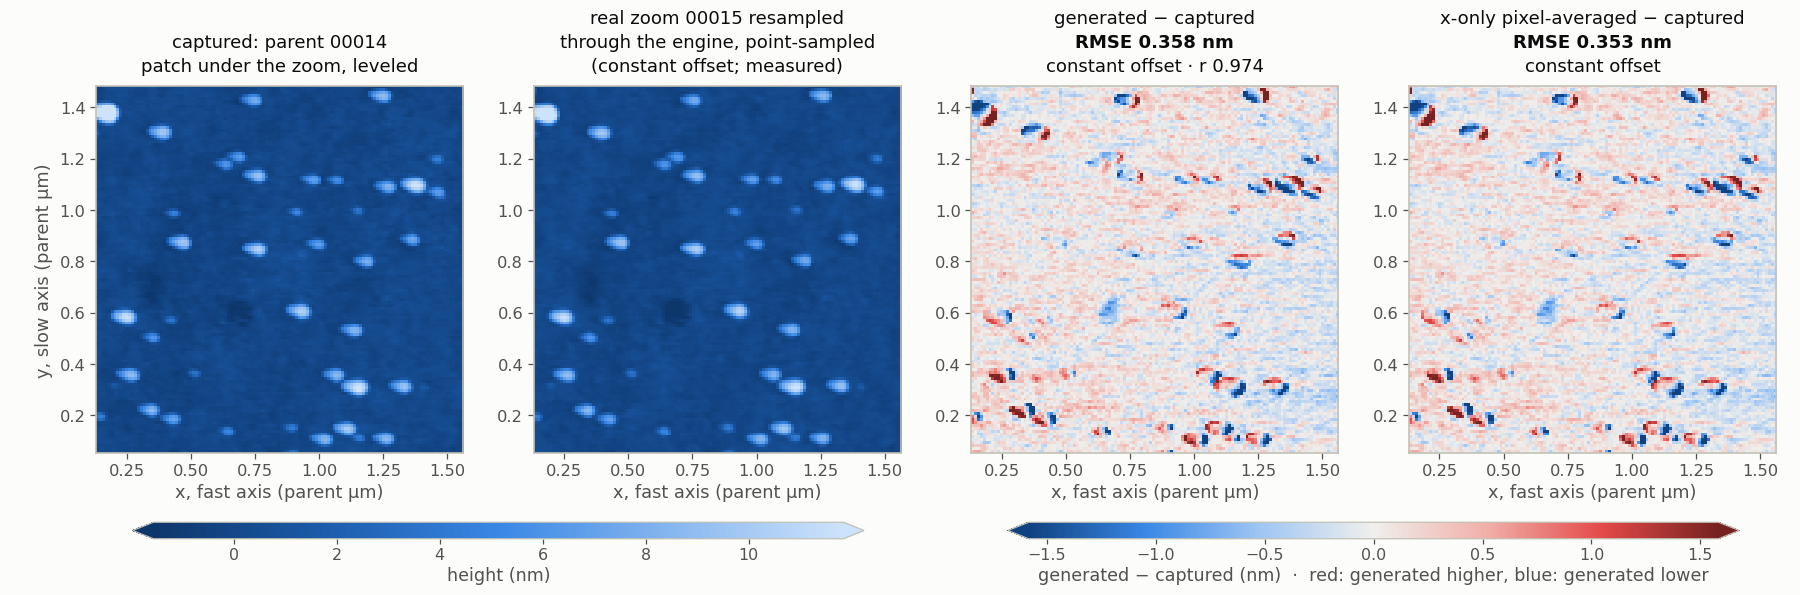
\includegraphics[width=\textwidth]{figures/psfilm_crossscale.png}
\caption{Cross-scale test on PSFILM (Icon, ScanAsyst-Air). From left: parent frame 00014 under the
zoom (11.36~nm/pixel); the measured zoom 00015 (5.81~nm/pixel) resampled through the engine onto
the parent grid; their difference (RMSE 0.358~nm, $r=0.974$); the same with fast-axis-only pixel
averaging (0.353~nm). The test is measured against measured and does not depend on the tip at
these pixel sizes.}
\label{fig:crossscale}
\end{figure}

A different test uses only measured data. Each finer zoom, resampled through the engine onto its
parent frame (Fig.~\ref{fig:crossscale}), reproduces the parent to 0.28--0.50~nm (FSILICA),
0.20--0.72~nm (PSFILM) and 1.0--1.6~nm (PS-LDPE) RMS \tagi. This checks the decoding, including
per-file auto-ranged $Z$ scales (consistent to 2--3\,\%), the pixel conventions, the registration
and the resampling layer. It does not depend on the tip, because dilation changes these images by
less than the noise; on PS-LDPE the dilation is exactly zero at the recorded pixel sizes. On the
soft LDPE phase, part of the residual reflects the different PeakForce setpoints of zoom and
parent, which a geometric model cannot represent. Figure~\ref{fig:polymers} summarises both
comparisons.

\begin{figure}[t]
\centering
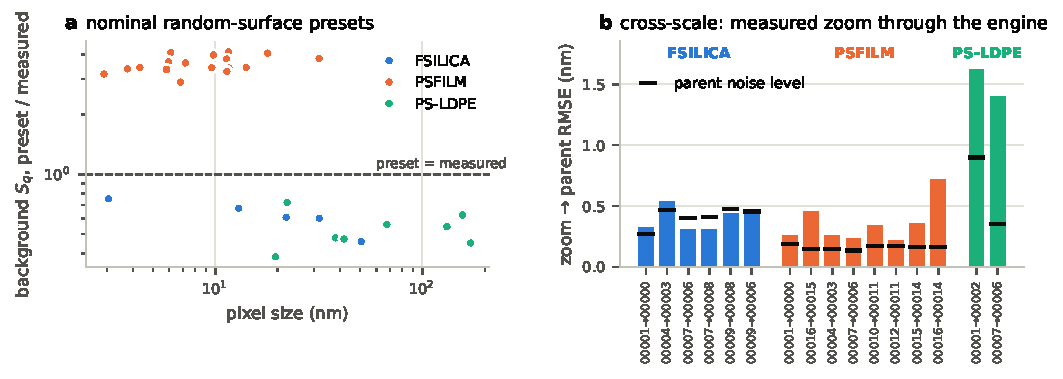
\includegraphics[width=\textwidth]{figures/fig_polymers.pdf}
\caption{Polymers and fused silica. (a) Background $S_q$ of the nominal random-surface preset,
simulated on each frame's grid with matched measurement noise, over the measured background $S_q$,
against pixel size (30 frames). (b) Cross-scale RMSE of each measured zoom resampled through the
engine onto its parent frame (16 pairs, child$\to$parent scan numbers), with the parent's noise
level. These values use the RMSE report's convention (one constant offset); the driver
convention with a fitted plane gives the slightly lower ranges quoted in the text.}
\label{fig:polymers}
\end{figure}

Robust blind tip reconstruction~\cite{villarrubia1997} on the tip-sensitive zooms excludes only
blunt apexes. On PSFILM an isotropic apex of 120~nm or more is excluded, but a blunt apex extended
only along $x$ is not. Every sharp candidate ($R\le12$~nm) passes, which demonstrates no power,
and every radius bound depends on the reconstruction's threshold settings \tagi.

\subsection{Negative control: the pipeline reports failed tracking instead of fitting it}

The two TGXYZ02 frames hold no tracked topography \tagm. In frame 00000 the $Z$ drive stayed at its
retract limit for the whole frame: every one of the 65,536 Height pixels holds the same limit
value, and every captured force curve lies within 0.95~nm of one template. In frame 00001 the
peak-force error is below $-\text{setpoint}/2$ in 84.7\,\% of pixels. The pipeline flags both
frames instead of fitting them. For the idealised model its sphere-on-step images equal the
closed form to 0~nm, but neither frame matches any prediction, and this mismatch says nothing
about the simulator.

%% =====================================================================
\section{Discussion}
\label{sec:discussion}

\subsection{What was validated}

Within its geometric assumptions, the simulator, given a measured sample model and a probe of
roughly the right size, reproduces real grating images at held-out sites to a few nanometres. The
remaining misfit lies on the walls, and identifiable instrument effects explain much of it. The
engine is identical to the browser page, its dilation equals closed forms where they exist, and
its decoding, pixel conventions and resampling are consistent across scales on real data.

\subsection{What these data cannot validate}

The same measurements bound the claims that can be made:
\begin{enumerate}
  \item \emph{Tip geometry at the nominal scale} ($R\lesssim12$~nm). No folder resolves it: grating
        walls are shallower than every facet, the polymer and fused-silica zooms give
        non-rejections without power, and PS-LDPE is pixel-limited. Only blunt apexes are excluded.
  \item \emph{Yaw sign and cantilever axis}, which centrosymmetric pits cannot reveal.
  \item \emph{Absolute $XY$ and $Z$ calibration}. No traceable standard was available; the
        scale factors found are session values.
  \item \emph{Feedback dynamics, holder tilt, mechanics and force-dependent indentation}, which
        are outside the model.
\end{enumerate}
A benchmark that reports agreement on these samples should therefore not be read as evidence
that the simulator's tip models are correct at the nanometre scale.

\subsection{Implications for simulator-based inverse methods}

Three practical points follow for anyone who trains or tests reconstruction methods on simulated
data.
\begin{enumerate}
  \item \emph{Header metadata is not ground truth.} The nominal probe radius in the file header was
        contradicted twice: by a factor of about 65 for the sphere probe, and for the 125~nm
        RTESPA apex relative to its cross-probe partner. Folder labels also conflict with headers
        (``SNL10 B'' against an RTESPA-300-like header). Independent probe characterisation
        (SEM, certificates, tip-check samples) is a prerequisite, not an option.
  \item \emph{Pixel response belongs in the forward model.} The instrument behaves as if each
        pixel were averaged over about one pixel along the fast axis. Ignoring this inflates an
        inferred radius about threefold, from 153 to 476~nm on CS-20NG.
  \item \emph{Samples must be tip-sensitive at the scale of interest.} Micrometre gratings with
        shallow walls validate sample models and registration, not tips. A validation of tip
        effects needs features sharper than the probe at the nanometre scale, imaged at pixel
        sizes comparable to the apex radius.
\end{enumerate}

\subsection{Limitations}

Each grating folder has only 1--3 held-out frames at 1--3 independent sites; one VGRP-GS hold-out
probably re-images the calibrate pits, and the SNL10 B hold-out is one field imaged twice. The
in-folder tip discrimination is a heuristic ratio, not a statistical test, and the cross-probe
rule cannot reach ``inconsistent'' at the available site counts. Quoted uncertainties are
within-session repeatability. Widths and corner radii depend on the estimator by 10--30~nm. Probe
identities are unverified: there was no SEM image, certificate or thermal tune.

%% =====================================================================
\section{Conclusions}
\label{sec:conclusions}

We validated an open, geometric AFM tip-convolution simulator against 51 real Bruker frames from
ten folders, using held-out frames, candidate-probe sweeps, a no-tip control, evidence tags and
independent verification of every headline claim. A measured grating model transferred to
held-out sites reproduces the images to 2.8--6.3~nm RMS, 5--18 times lower than the nominal
presets. The same data reject the probe radius stated in the file headers and show that the
fast-axis pixel response must be modelled. They do not identify the tip at the nanometre scale,
the yaw, or the absolute calibration. These limits are the boundary conditions for the next step,
the inverse problem: recovering known calibration geometry from real scans, with reconstruction
quality measured against independently characterised probes.

%% =====================================================================
\section*{Code and data availability}
The simulator (browser applications and Python engine), the validation pipeline, the case
catalogue and the tests are available at \todo{repository URL / DOI}. The raw Bruker data are
\todo{available from the authors on request / deposited at \ldots}.

\section*{CRediT authorship contribution statement}
\todo{Fill in per author: Conceptualization, Software, Validation, Formal analysis, Writing.}

\section*{Declaration of competing interest}
\todo{The authors declare that they have no known competing financial interests or personal
relationships that could have appeared to influence the work reported in this paper.}

\section*{Acknowledgements}
\todo{Instrument operators, facility, funding.}

\bibliographystyle{elsarticle-num}
\bibliography{references}

\end{document}
